% This is based on "sig-alternate.tex" V2.0 May 2012
% This file should be compiled with V2.5 of "sig-alternate.cls" May 2012
%
% ----------------------------------------------------------------------------------------------------------------
%
% This .tex source is an example which *does* use
% the .bib file (from which the .bbl file % is produced).
% REMEMBER HOWEVER: After having produced the .bbl file,
% and prior to final submission, you *NEED* to 'insert'
% your .bbl file into your source .tex file so as to provide
% ONE 'self-contained' source file.
%
% Information on the sig-alternate class file and on the
% GECCO workshop paper format and submission can be found at these
% locations:
% http://www.acm.org/sigs/publications/proceedings-templates#aL2
% http://www.sheridanprinting.com/typedept/gecco3.htm
%
% ================= IF YOU HAVE QUESTIONS =======================
% Questions regarding the SIGS styles, SIGS policies and
% procedures, Conferences etc. should be sent to
% Adrienne Griscti (griscti@acm.org)
%
% Technical questions to bbob@lri.fr
% ===============================================================
%

\documentclass{sig-alternate}
\pdfpagewidth=8.5in
\pdfpageheight=11in
\special{papersize=8.5in,11in}

%%%%%%%%%%%%%%%%%%%%%%%%%%%%%%%%%%%%%%%%%%%%%%%%%%%%%%
% Packages
\usepackage{graphicx}
\usepackage{tabularx}
\usepackage[dvipsnames]{xcolor}
\usepackage{float}
\usepackage{rotating}
\usepackage{xstring} % for string operations
\usepackage{wasysym} % Table legend with symbols input from post-processing
\usepackage{MnSymbol} % Table legend with symbols input from post-processing

%%%%%%%%%%%%%%%%%%%%%%%%%%%%%%%%%%%%%%%%%%%%%%%%%%%%%%
% Definitions

% Algorithm names on the right of the ECDF figures can be modified by
% uncommenting the following lines and inputting some text in the last
% brackets, make sure the algorithms are in the same order as for the post-processing:
% \newcommand{\algaperfprof}{Algorithm a short name}
% \newcommand{\algbperfprof}{Algorithm b short name}
% \newcommand{\algcperfprof}{Algorithm c short name}
% \newcommand{\algdperfprof}{Algorithm c short name}
% ...
% Algorithm names as they appear in the tables, uncomment if necessary
% \newcommand{\algatables}{\algaperfprof}  % first argument in the post-processing
% \newcommand{\algbtables}{\algbperfprof}  % first argument in the post-processing
% \newcommand{\algctables}{\algcperfprof}  % first argument in the post-processing
% \newcommand{\algdtables}{\algdperfprof}  % second argument in the post-processing
% ...
% location of pictures files
\newcommand{\bbobdatapath}{ppdata/}
\input{\bbobdatapath bbob_pproc_commands.tex}
\graphicspath{{\bbobdatapath}}

%%%%%%%%%%%%%%%%%%%%%%%%%%%%%%%%%%%%%%%%%%%%%%%%%%%%%%
% pre-defined commands
\newcommand{\DIM}{\ensuremath{\mathrm{DIM}}}
\newcommand{\ERT}{\ensuremath{\mathrm{ERT}}}
\newcommand{\FEvals}{\ensuremath{\mathrm{FEvals}}}
\newcommand{\nruns}{\ensuremath{\mathrm{Nruns}}}
\newcommand{\Dfb}{\ensuremath{\Delta f_{\mathrm{best}}}}
\newcommand{\Df}{\ensuremath{\Delta f}}
\newcommand{\nbFEs}{\ensuremath{\mathrm{\#FEs}}}
\newcommand{\fopt}{\ensuremath{f_\mathrm{opt}}}
\newcommand{\ftarget}{\ensuremath{f_\mathrm{t}}}
\newcommand{\CrE}{\ensuremath{\mathrm{CrE}}}
\newcommand{\change}[1]{{\color{red} #1}}

    \renewcommand{\topfraction}{1}	% max fraction of floats at top
    \renewcommand{\bottomfraction}{1} % max fraction of floats at bottom
    %   Parameters for TEXT pages (not float pages):
    \setcounter{topnumber}{3}
    \setcounter{bottomnumber}{3}
    \setcounter{totalnumber}{3}     % 2 may work better
    \setcounter{dbltopnumber}{4}    % for 2-column pages
    \renewcommand{\dbltopfraction}{1}	% fit big float above 2-col. text
    \renewcommand{\textfraction}{0.0}	% allow minimal text w. figs
    %   Parameters for FLOAT pages (not text pages):
    \renewcommand{\floatpagefraction}{0.80}	% require fuller float pages
    % N.B.: floatpagefraction MUST be less than topfraction !!
    \renewcommand{\dblfloatpagefraction}{0.7}	% require fuller float pages

%%%%%%%%%%%%%%%%%%%%%%%%%%%%%%%%%%%%%%%%%%%%%%%%%%%%%%

\begin{document}


%
% --- Author Metadata here ---
\conferenceinfo{GECCO'13,} {July 6-10, 2013, Amsterdam, The Netherlands.}
\CopyrightYear{2013}
\crdata{TBA}
\clubpenalty=10000
\widowpenalty = 10000
% --- End of Author Metadata ---

\title{Black-Box Optimization Benchmarking Template for the Comparison of More than Two Algorithms on the Noiseless Testbed}
\subtitle{Draft version
\titlenote{Submission deadline: March 28th.}}
%Camera-ready paper due April 16th.}}

%
% You need the command \numberofauthors to handle the 'placement
% and alignment' of the authors beneath the title.
%
% For aesthetic reasons, we recommend 'three authors at a time'
% i.e. three 'name/affiliation blocks' be placed beneath the title.
%
% NOTE: You are NOT restricted in how many 'rows' of
% "name/affiliations" may appear. We just ask that you restrict
% the number of 'columns' to three.
%
% Because of the available 'opening page real-estate'
% we ask you to refrain from putting more than six authors
% (two rows with three columns) beneath the article title.
% More than six makes the first-page appear very cluttered indeed.
%
% Use the \alignauthor commands to handle the names
% and affiliations for an 'aesthetic maximum' of six authors.
% Add names, affiliations, addresses for
% the seventh etc. author(s) as the argument for the
% \additionalauthors command.
% These 'additional authors' will be output/set for you
% without further effort on your part as the last section in
% the body of your article BEFORE References or any Appendices.

\numberofauthors{1} %  in this sample file, there are a *total*
% of EIGHT authors. SIX appear on the 'first-page' (for formatting
% reasons) and the remaining two appear in the \additionalauthors section.
%
\author{
% You can go ahead and credit any number of authors here,
% e.g. one 'row of three' or two rows (consisting of one row of three
% and a second row of one, two or three).
%
% The command \alignauthor (no curly braces needed) should
% precede each author name, affiliation/snail-mail address and
% e-mail address. Additionally, tag each line of
% affiliation/address with \affaddr, and tag the
% e-mail address with \email.
%
% 1st. author
\alignauthor
Forename Name\\ %\titlenote{Dr.~Trovato insisted his name be first.}\\
%       \affaddr{Institute for Clarity in Documentation}\\
%       \affaddr{1932 Wallamaloo Lane}\\
%       \affaddr{Wallamaloo, New Zealand}\\
%       \email{trovato@corporation.com}
%% 2nd. author
%\alignauthor
%G.K.M. Tobin\titlenote{The secretary disavows
%any knowledge of this author's actions.}\\
%       \affaddr{Institute for Clarity in Documentation}\\
%       \affaddr{P.O. Box 1212}\\
%       \affaddr{Dublin, Ohio 43017-6221}\\
%       \email{webmaster@marysville-ohio.com}
%% 3rd. author
%\alignauthor Lars Th{\o}rv{\"a}ld\titlenote{This author is the
%one who did all the really hard work.}\\
%       \affaddr{The Th{\o}rv{\"a}ld Group}\\
%       \affaddr{1 Th{\o}rv{\"a}ld Circle}\\
%       \affaddr{Hekla, Iceland}\\
%       \email{larst@affiliation.org}
%\and  % use '\and' if you need 'another row' of author names
%% 4th. author
%\alignauthor Lawrence P. Leipuner\\
%       \affaddr{Brookhaven Laboratories}\\
%       \affaddr{Brookhaven National Lab}\\
%       \affaddr{P.O. Box 5000}\\
%       \email{lleipuner@researchlabs.org}
%% 5th. author
%\alignauthor Sean Fogarty\\
%       \affaddr{NASA Ames Research Center}\\
%       \affaddr{Moffett Field}\\
%       \affaddr{California 94035}\\
%       \email{fogartys@amesres.org}
%% 6th. author
%\alignauthor Charles Palmer\\
%       \affaddr{Palmer Research Laboratories}\\
%       \affaddr{8600 Datapoint Drive}\\
%       \affaddr{San Antonio, Texas 78229}\\
%       \email{cpalmer@prl.com}
} % author
%% There's nothing stopping you putting the seventh, eighth, etc.
%% author on the opening page (as the 'third row') but we ask,
%% for aesthetic reasons that you place these 'additional authors'
%% in the \additional authors block, viz.
%\additionalauthors{Additional authors: John Smith (The Th{\o}rv{\"a}ld Group,
%email: {\texttt{jsmith@affiliation.org}}) and Julius P.~Kumquat
%(The Kumquat Consortium, email: {\texttt{jpkumquat@consortium.net}}).}
%\date{30 July 1999}
%% Just remember to make sure that the TOTAL number of authors
%% is the number that will appear on the first page PLUS the
%% number that will appear in the \additionalauthors section.

\maketitle
\begin{abstract}
to be written
\end{abstract}

% Add any ACM category that you feel is needed
\category{G.1.6}{Numerical Analysis}{Optimization}[global optimization,
unconstrained optimization]
\category{F.2.1}{Analysis of Algorithms and Problem Complexity}{Numerical Algorithms and Problems}

% Complete with anything that is needed
\terms{Algorithms}

% Complete with anything that is needed
\keywords{Benchmarking, Black-box optimization}

% \section{Introduction}
%
% \section{Algorithm Presentation}
%
% \section{Experimental Procedure}
%
%%%%%%%%%%%%%%%%%%%%%%%%%%%%%%%%%%%%%%%%%%%%%%%%%%%%%%%%%%%%%%%%%%%%%%%%%%%%%%%
\section{CPU Timing}
%%%%%%%%%%%%%%%%%%%%%%%%%%%%%%%%%%%%%%%%%%%%%%%%%%%%%%%%%%%%%%%%%%%%%%%%%%%%%%%
% note that the following text is just a proposal and can/should be changed to your needs:
In order to evaluate the CPU timing of the algorithm, we have run the \change{MY-ALGORITHM-NAME} on the function $f_{8}$ with restarts for at least 30 seconds and until a maximum budget equal to \change{$400 (D + 2)$} is reached. The code was run on a \change{Mac Intel(R) Core(TM) i5-2400S CPU @ 2.50GHz} with \change{1} processor and \change{4} cores. The time per function evaluation for dimensions 2, 3, 5, 10, 20\change{, 40} equals \change{$x.x$}, \change{$x.x$}, \change{$x.x$}, \change{$xx$}, \change{$xxx$}\change{, and $xxx$} milliseconds respectively. 

\change{repeat the above for any algorithm tested}


%%%%%%%%%%%%%%%%%%%%%%%%%%%%%%%%%%%%%%%%%%%%%%%%%%%%%%%%%%%%%%%%%%%%%%%%%%%%%%%
\section{Results}
%%%%%%%%%%%%%%%%%%%%%%%%%%%%%%%%%%%%%%%%%%%%%%%%%%%%%%%%%%%%%%%%%%%%%%%%%%%%%%%

Results from experiments according to \cite{hansen2012exp} on the
benchmark functions given in \cite{wp200901_2010,hansen2012fun} are
presented in Figures~\ref{fig:scaling}, \ref{fig:ECDFs05D} and
\ref{fig:ECDFs20D} and in Tables~\ref{tab:ERTs5} and~\ref{tab:ERTs20}. The
\textbf{expected running time (ERT)}, used in the figures and tables,
depends on a given target function value, $\ftarget=\fopt+\Df$, and is
computed over all relevant trials as the number of function
evaluations executed during each trial while the best function value
did not reach \ftarget, summed over all trials and divided by the
number of trials that actually reached \ftarget\
\cite{hansen2012exp,price1997dev}.  \textbf{Statistical significance}
is tested with the rank-sum test for a given target $\Delta\ftarget$
%($10^{-8}$ as in Figure~\ref{fig:scaling})
using, for each trial,
either the number of needed function evaluations to reach
$\Delta\ftarget$ (inverted and multiplied by $-1$), or, if the target
was not reached, the best $\Df$-value achieved, measured only up to
the smallest number of overall function evaluations for any
unsuccessful trial under consideration.


%%%%%%%%%%%%%%%%%%%%%%%%%%%%%%%%%%%%%%%%%%%%%%%%%%%%%%%%%%%%%%%%%%%%%%%%%%%%%%%
%%%%%%%%%%%%%%%%%%%%%%%%%%%%%%%%%%%%%%%%%%%%%%%%%%%%%%%%%%%%%%%%%%%%%%%%%%%%%%%

% Scaling of ERT with dimension

%%%%%%%%%%%%%%%%%%%%%%%%%%%%%%%%%%%%%%%%%%%%%%%%%%%%%%%%%%%%%%%%%%%%%%%%%%%%%%%
\begin{figure*}
\centering
\begin{tabular}{@{}c@{}c@{}c@{}c@{}}
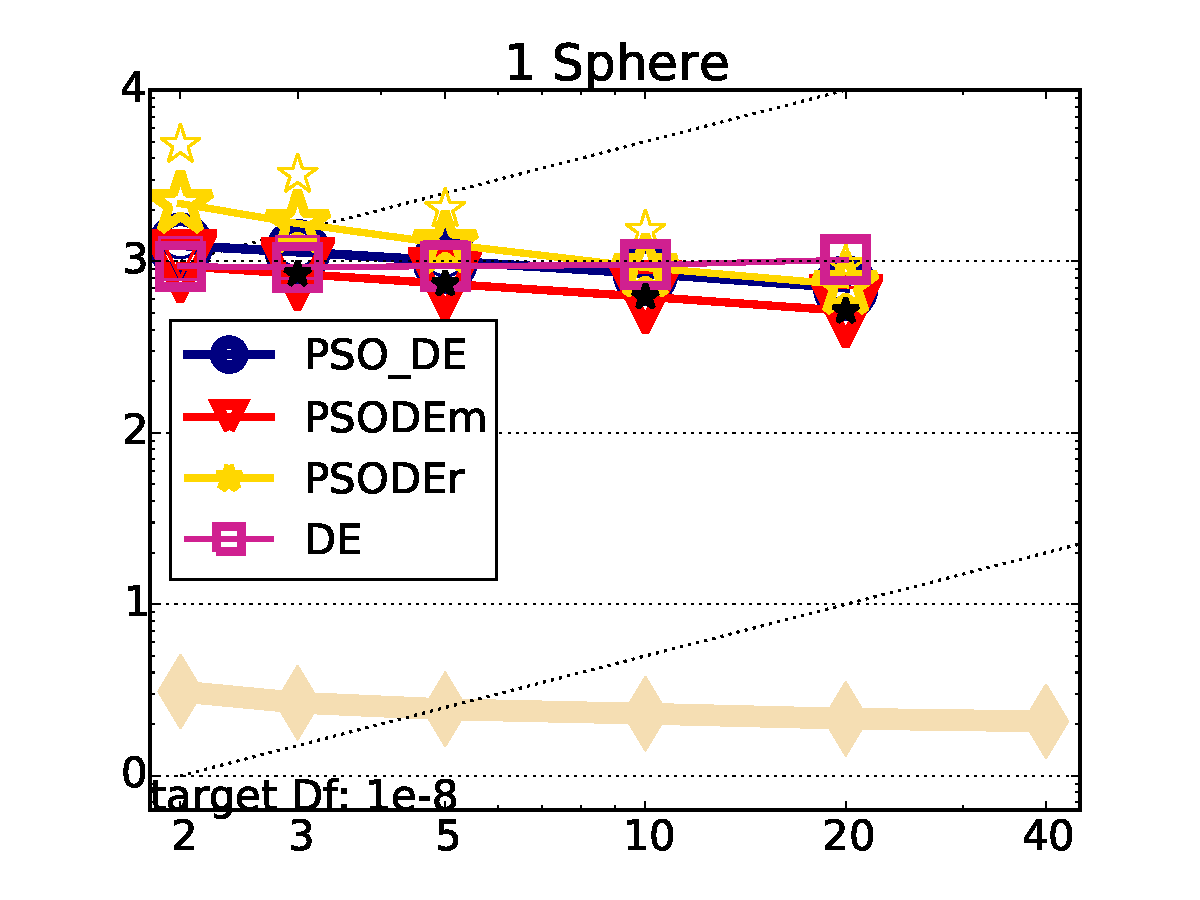
\includegraphics[width=0.253\textwidth, trim= 0.7cm 0.8cm 0.5cm 0.5cm, clip]{ppfigs_f001}&
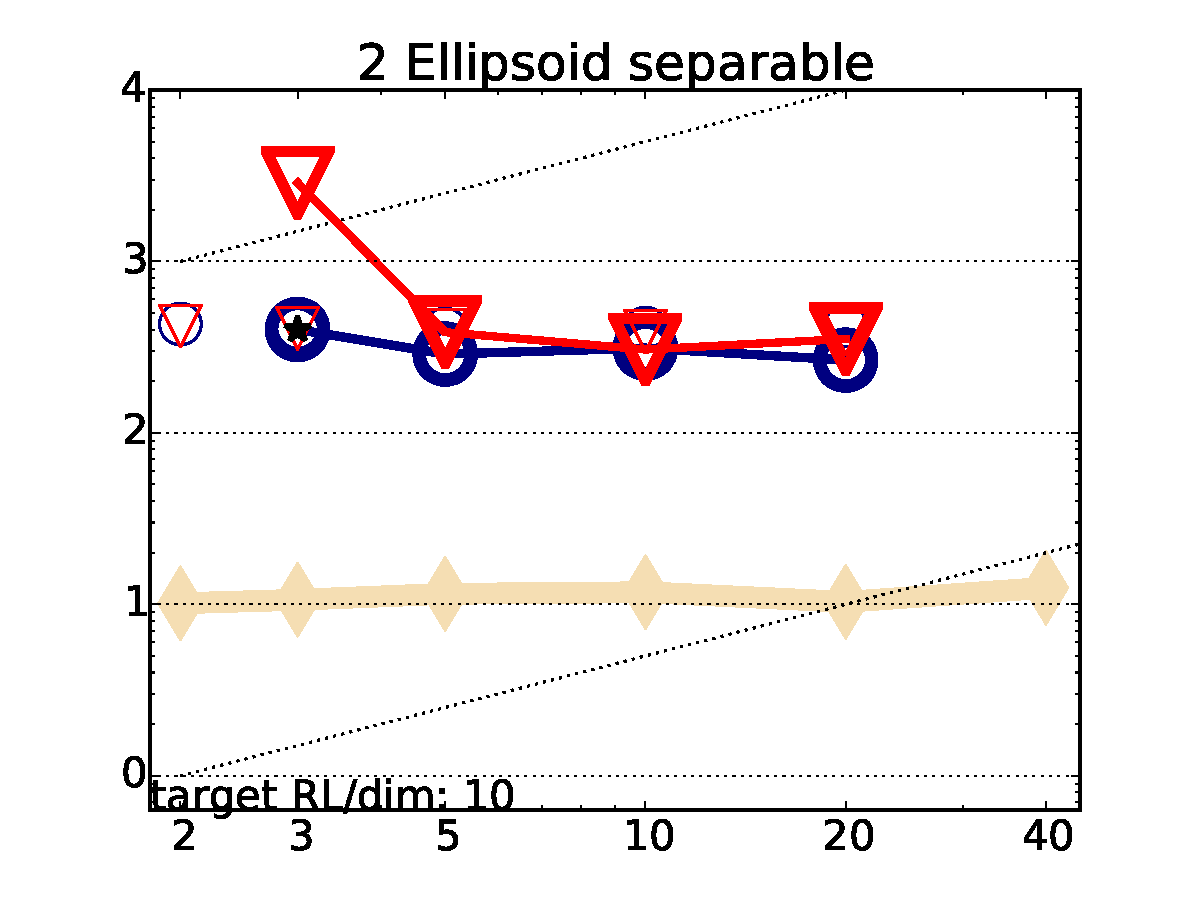
\includegraphics[width=0.238\textwidth, trim= 1.8cm 0.8cm 0.5cm 0.5cm, clip]{ppfigs_f002}&
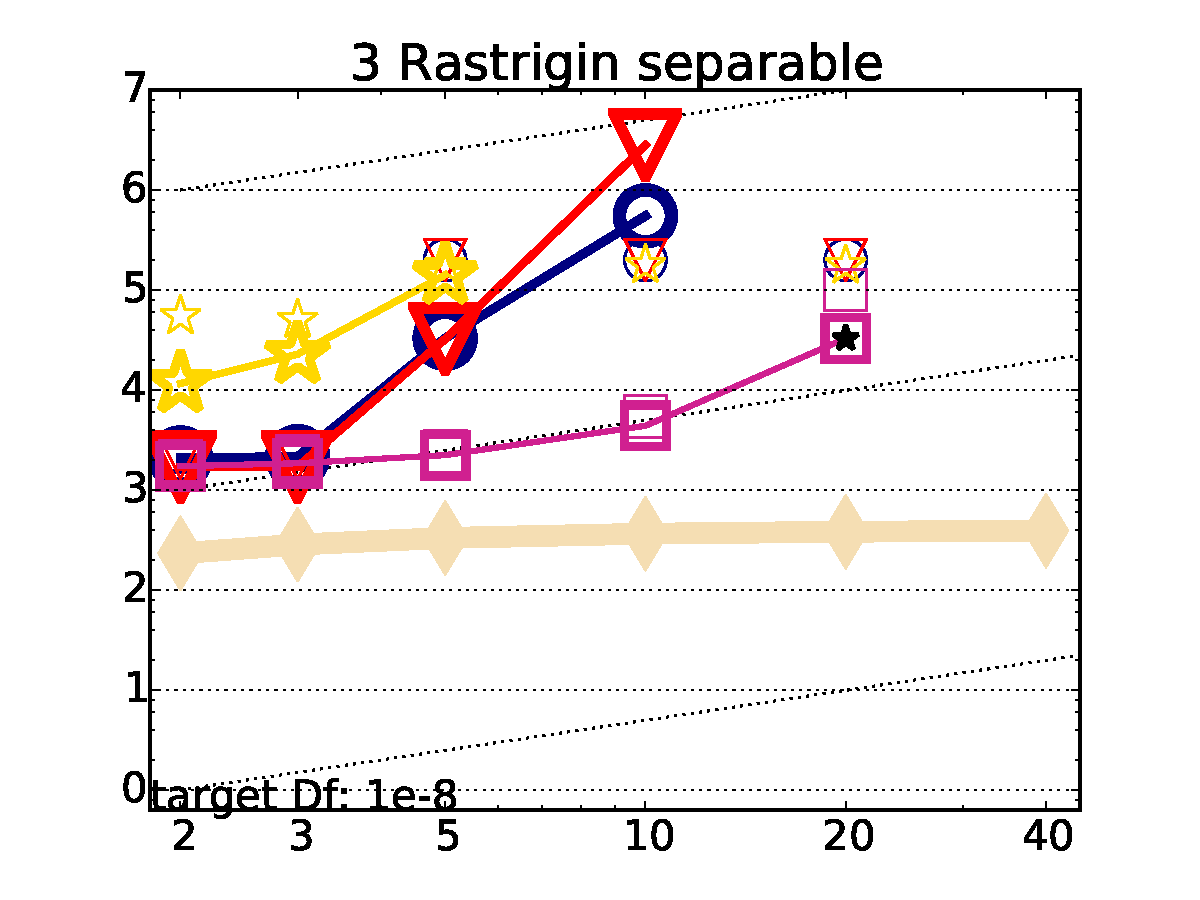
\includegraphics[width=0.238\textwidth, trim= 1.8cm 0.8cm 0.5cm 0.5cm, clip]{ppfigs_f003}&
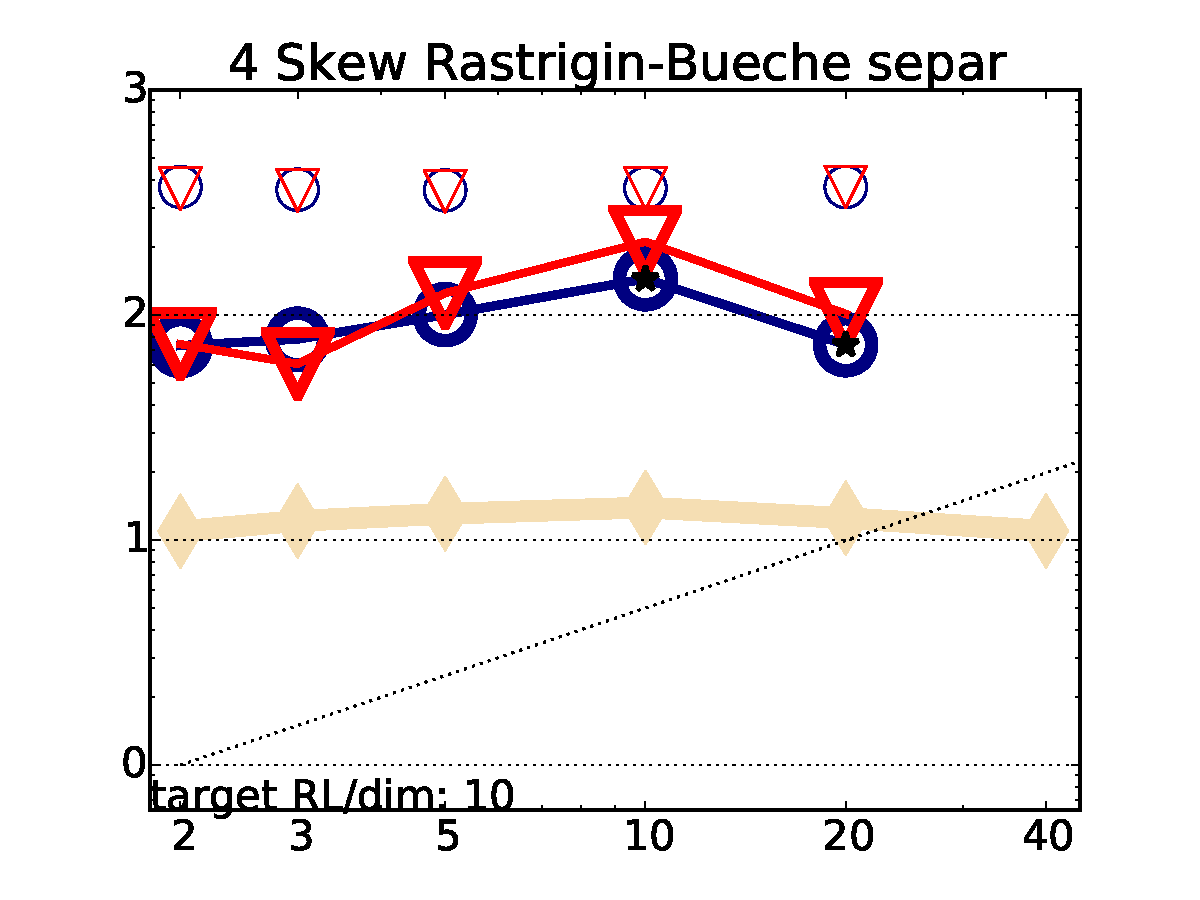
\includegraphics[width=0.238\textwidth, trim= 1.8cm 0.8cm 0.5cm 0.5cm, clip]{ppfigs_f004}\\
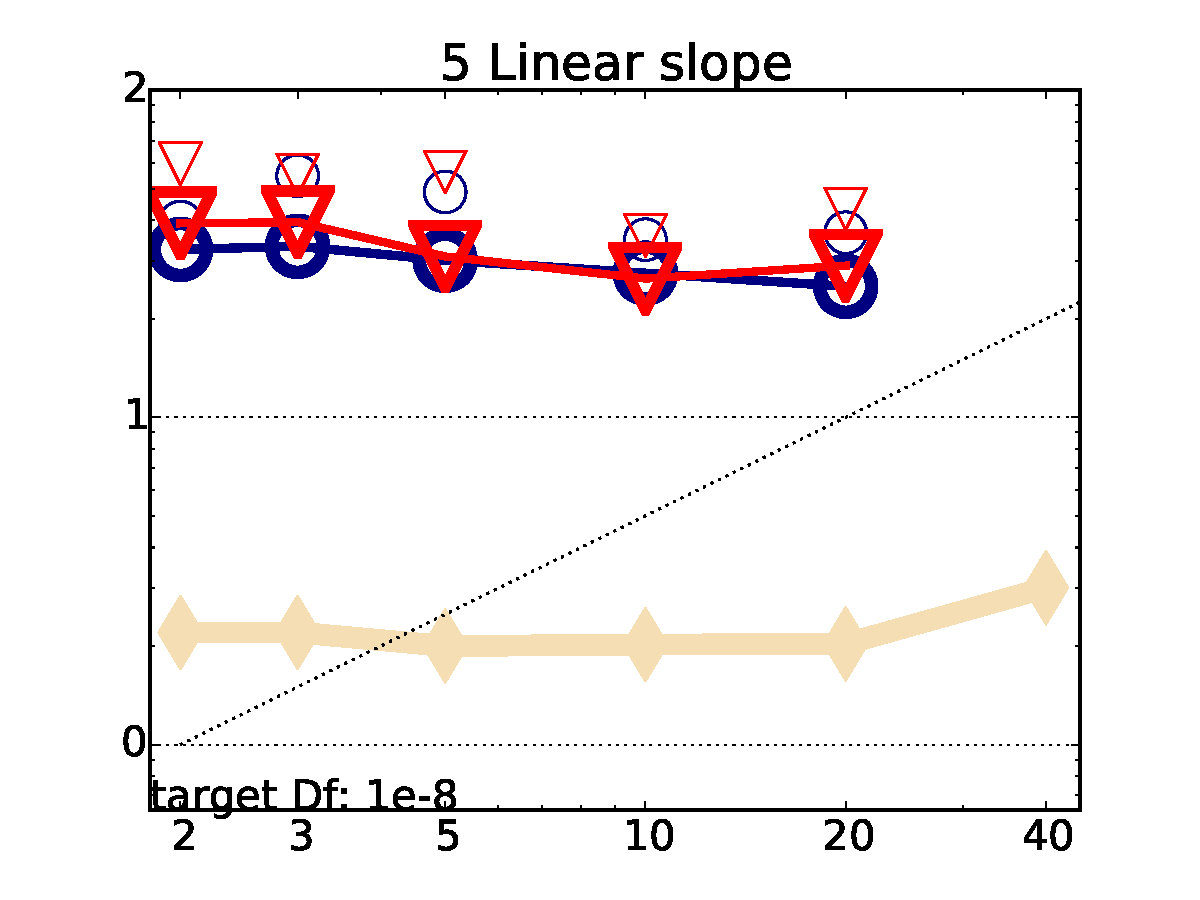
\includegraphics[width=0.253\textwidth, trim= 0.7cm 0.8cm 0.5cm 0.5cm, clip]{ppfigs_f005}&
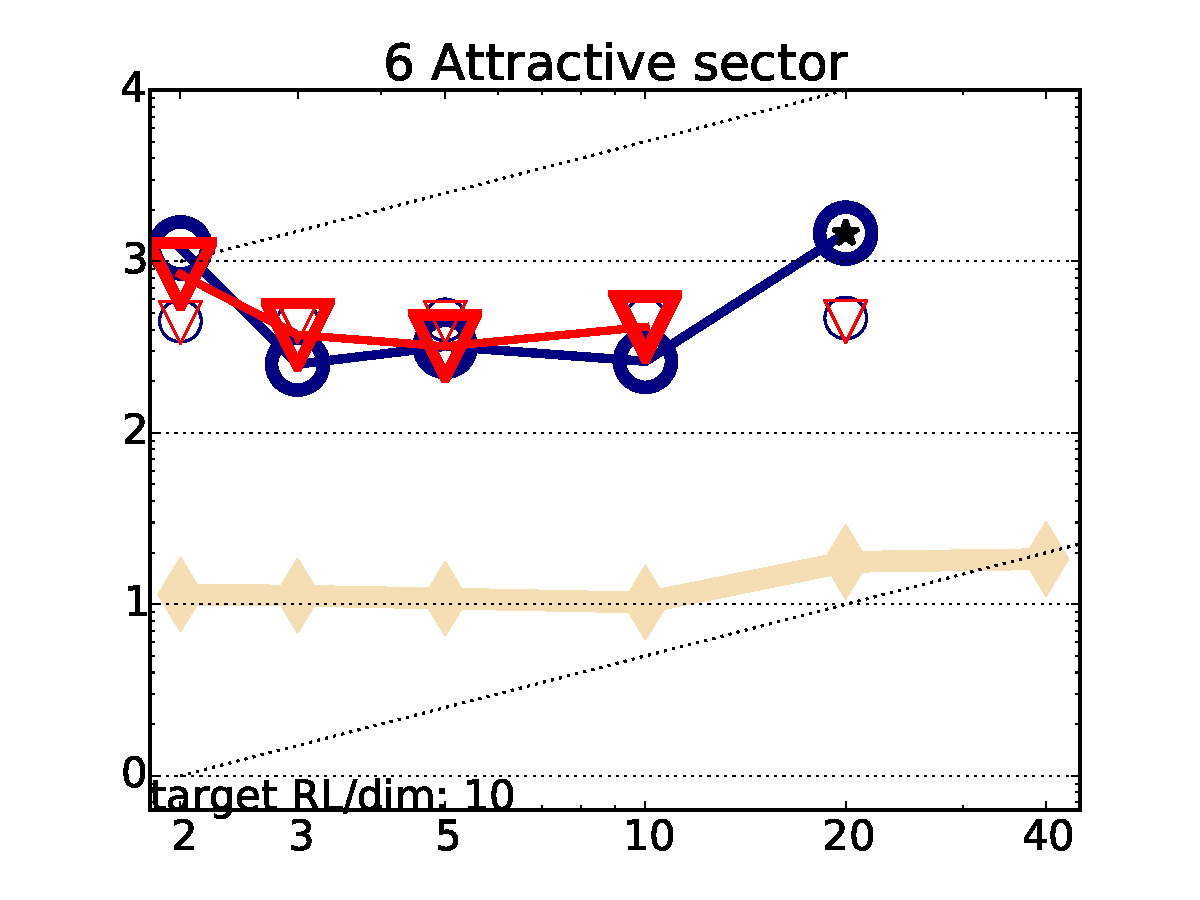
\includegraphics[width=0.238\textwidth, trim= 1.8cm 0.8cm 0.5cm 0.5cm, clip]{ppfigs_f006}&
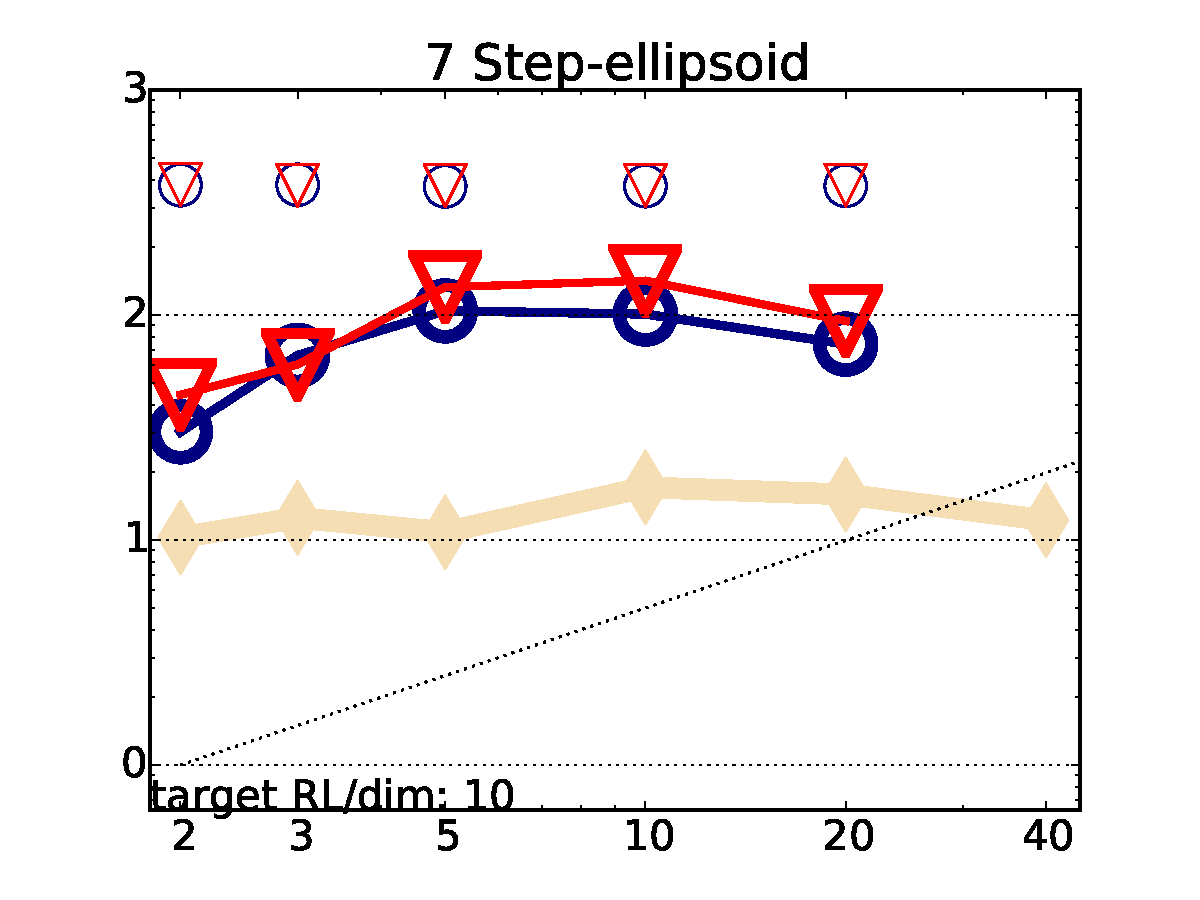
\includegraphics[width=0.238\textwidth, trim= 1.8cm 0.8cm 0.5cm 0.5cm, clip]{ppfigs_f007}&
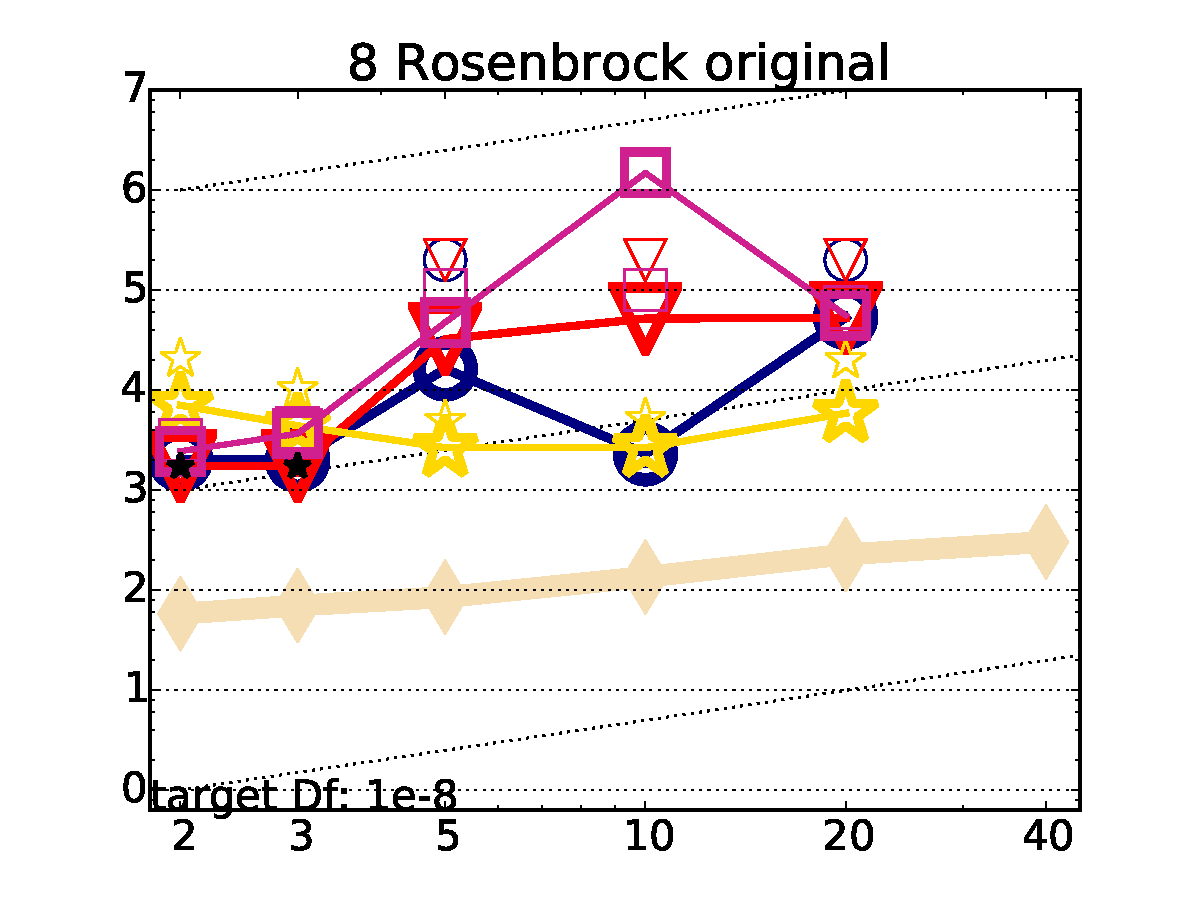
\includegraphics[width=0.238\textwidth, trim= 1.8cm 0.8cm 0.5cm 0.5cm, clip]{ppfigs_f008}\\
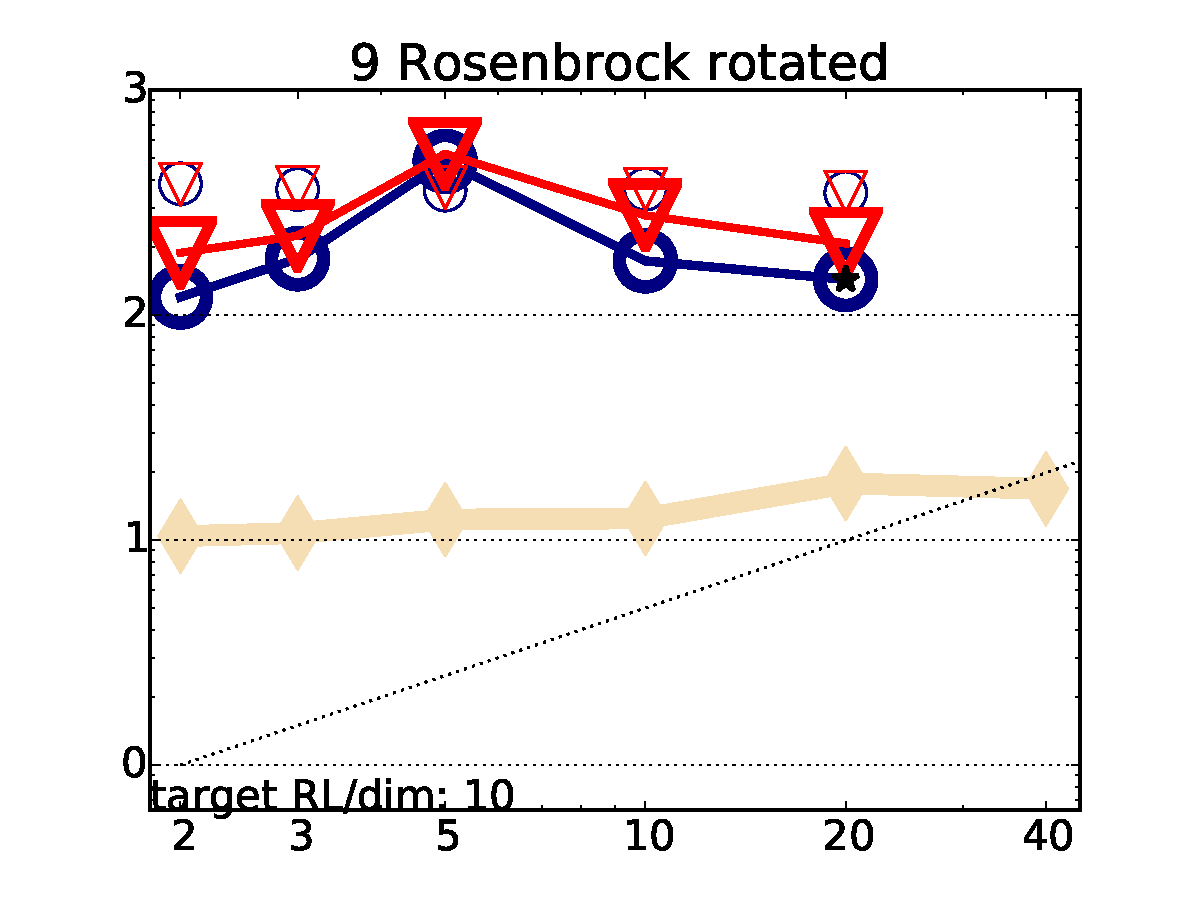
\includegraphics[width=0.253\textwidth, trim= 0.7cm 0.8cm 0.5cm 0.5cm, clip]{ppfigs_f009}&
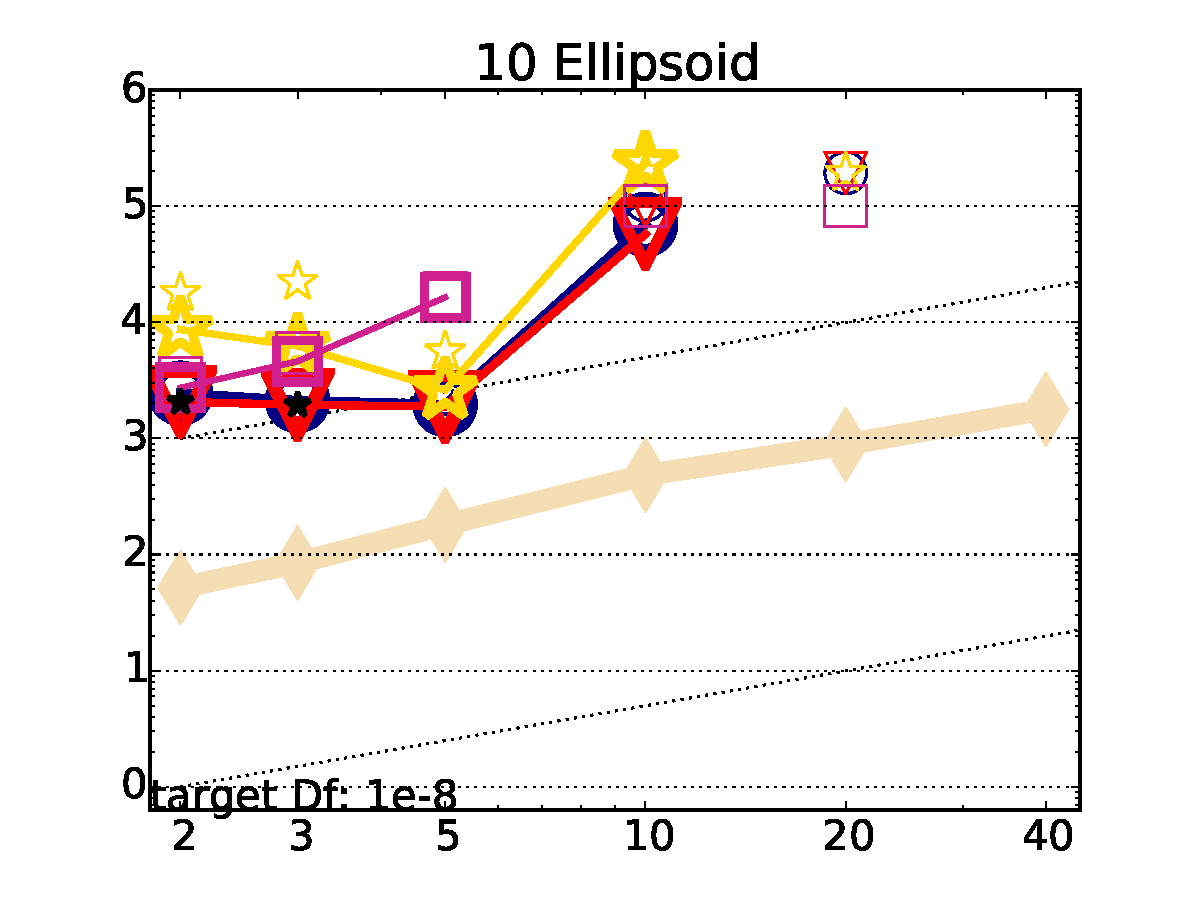
\includegraphics[width=0.238\textwidth, trim= 1.8cm 0.8cm 0.5cm 0.5cm, clip]{ppfigs_f010}&
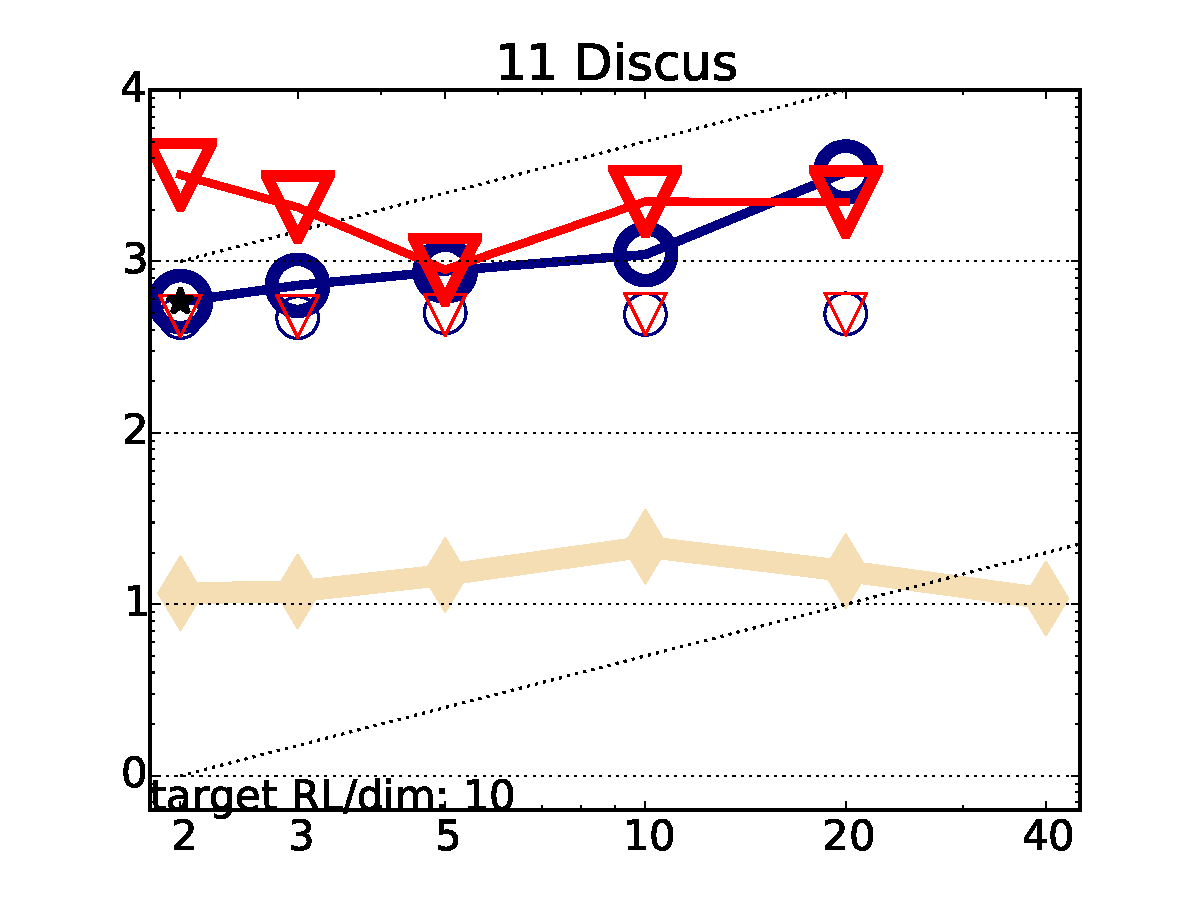
\includegraphics[width=0.238\textwidth, trim= 1.8cm 0.8cm 0.5cm 0.5cm, clip]{ppfigs_f011}&
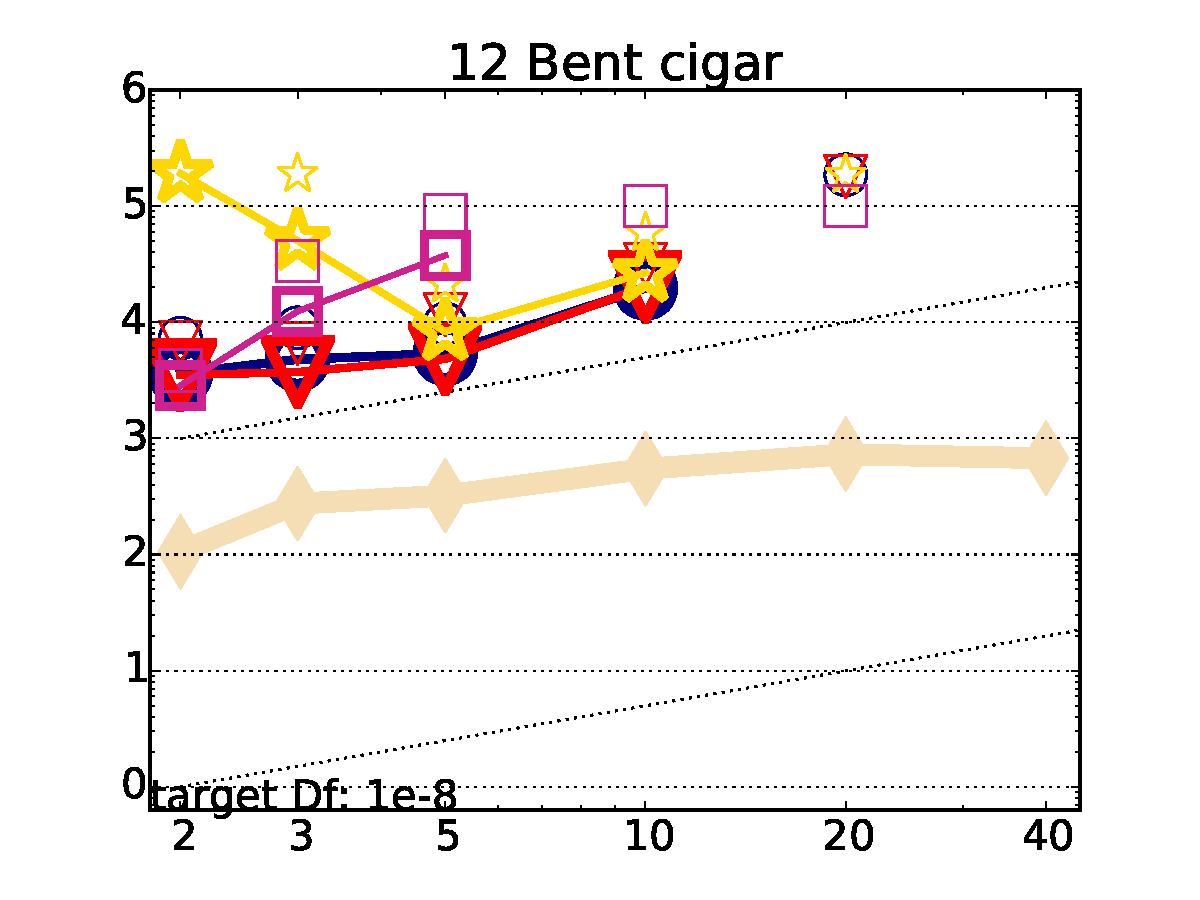
\includegraphics[width=0.238\textwidth, trim= 1.8cm 0.8cm 0.5cm 0.5cm, clip]{ppfigs_f012}\\
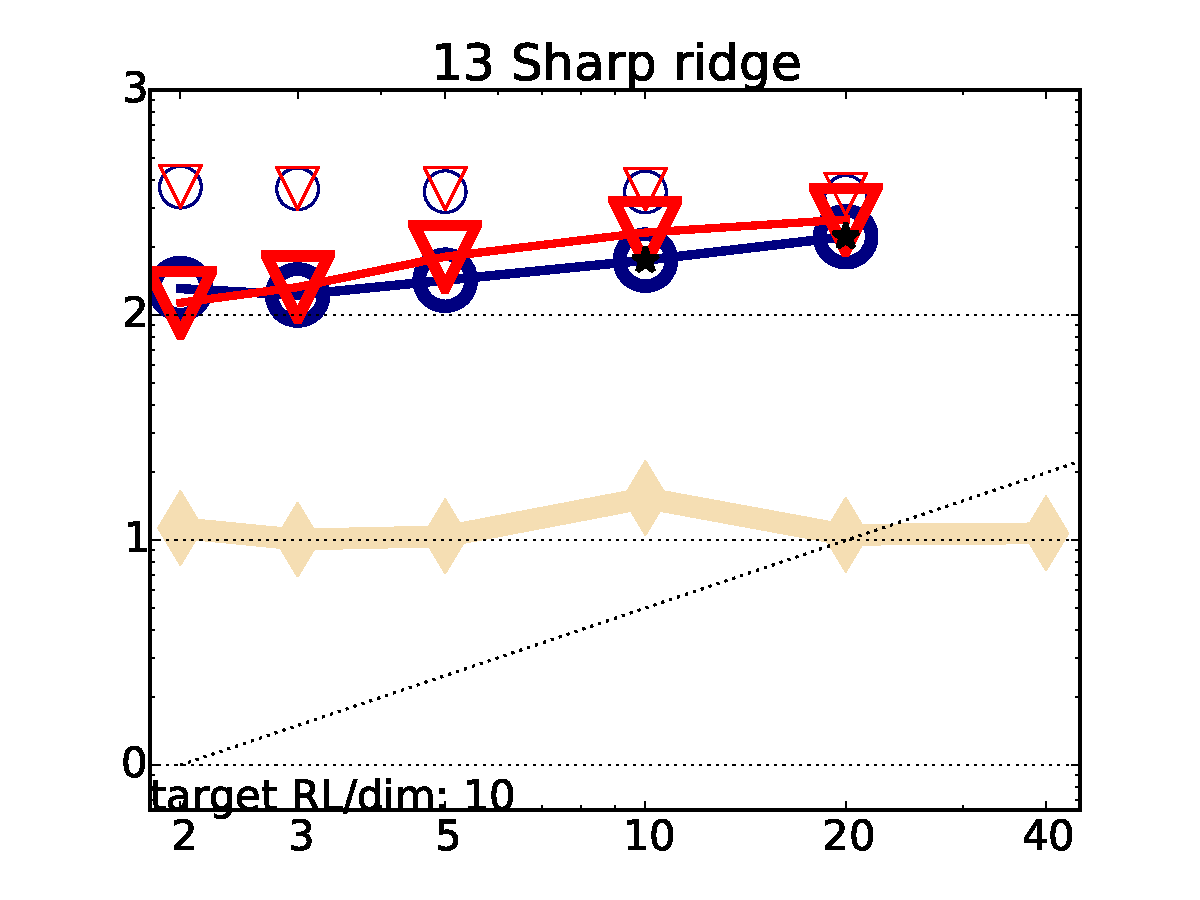
\includegraphics[width=0.253\textwidth, trim= 0.7cm 0.8cm 0.5cm 0.5cm, clip]{ppfigs_f013}&
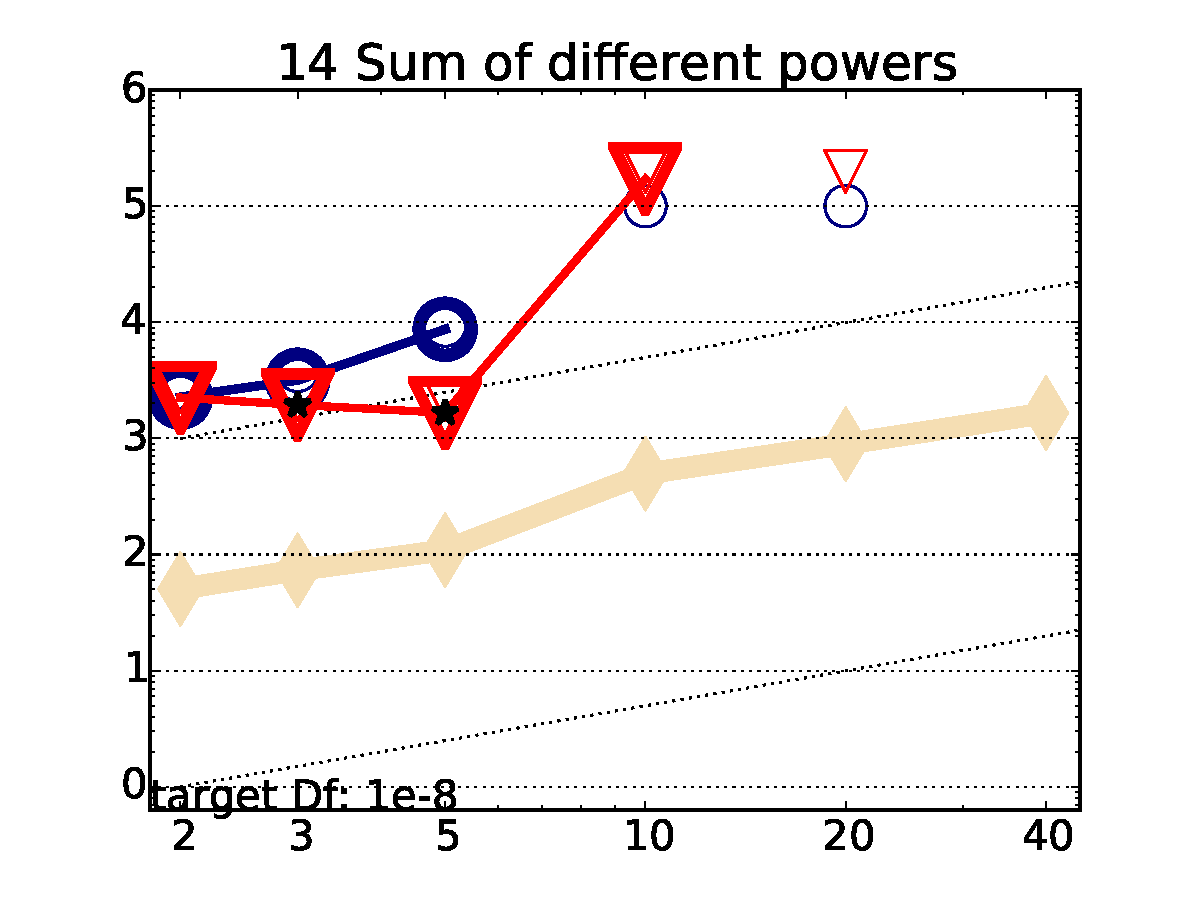
\includegraphics[width=0.238\textwidth, trim= 1.8cm 0.8cm 0.5cm 0.5cm, clip]{ppfigs_f014}&
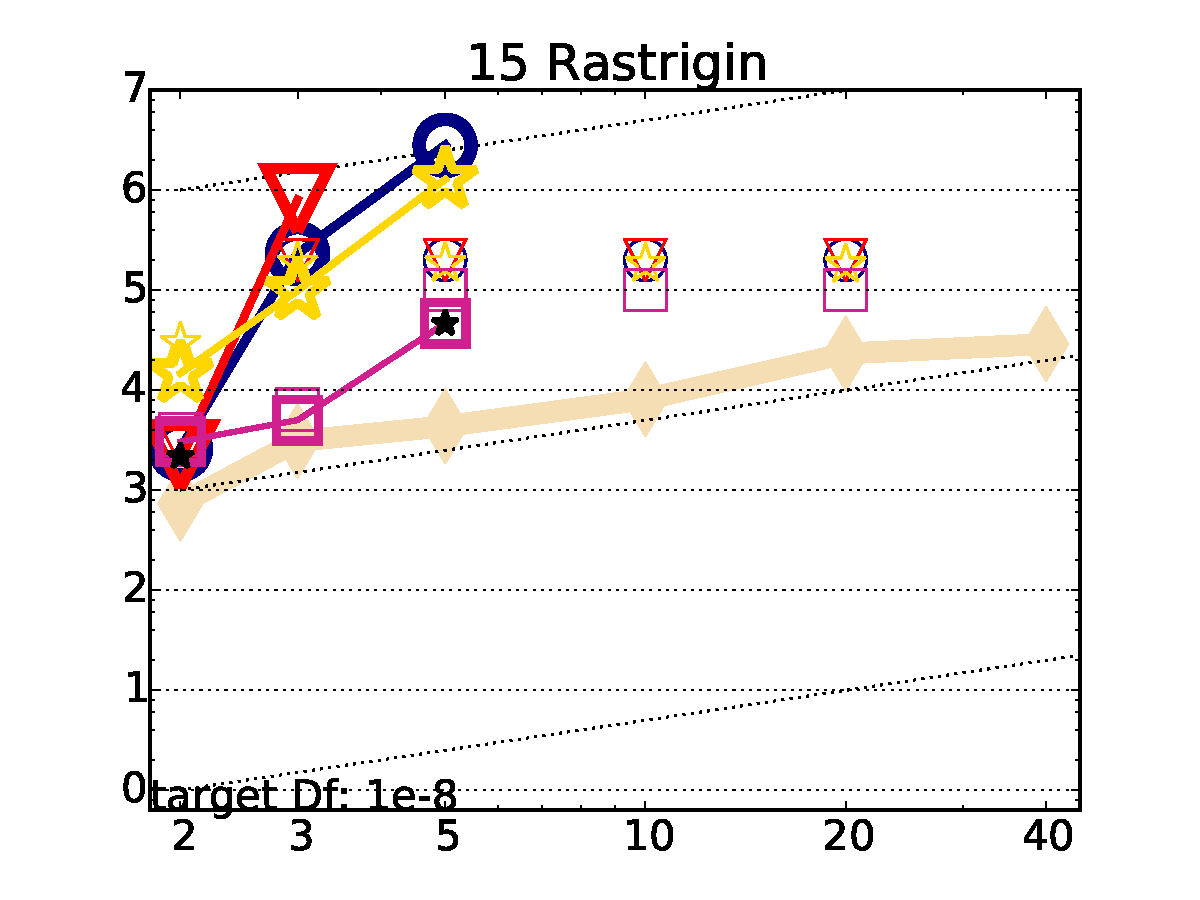
\includegraphics[width=0.238\textwidth, trim= 1.8cm 0.8cm 0.5cm 0.5cm, clip]{ppfigs_f015}&
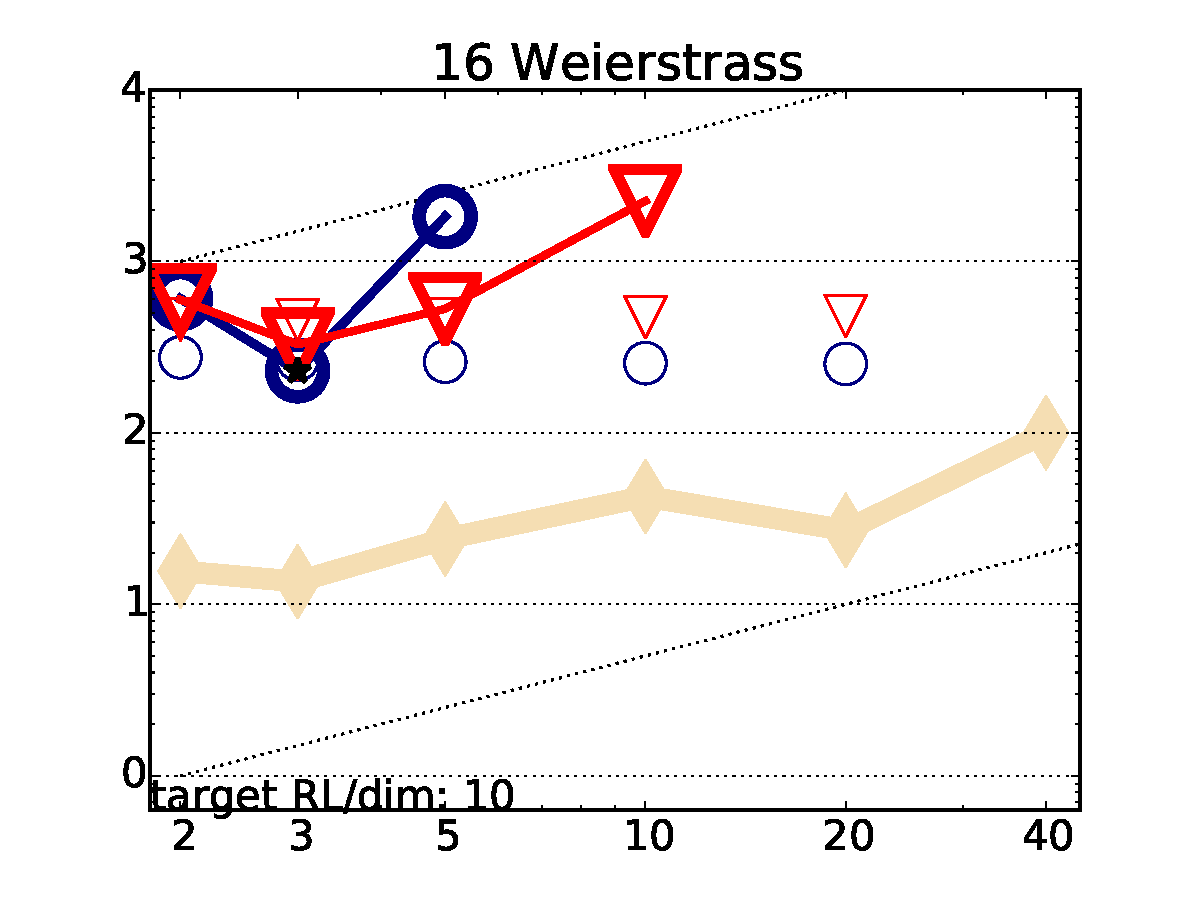
\includegraphics[width=0.238\textwidth, trim= 1.8cm 0.8cm 0.5cm 0.5cm, clip]{ppfigs_f016}\\
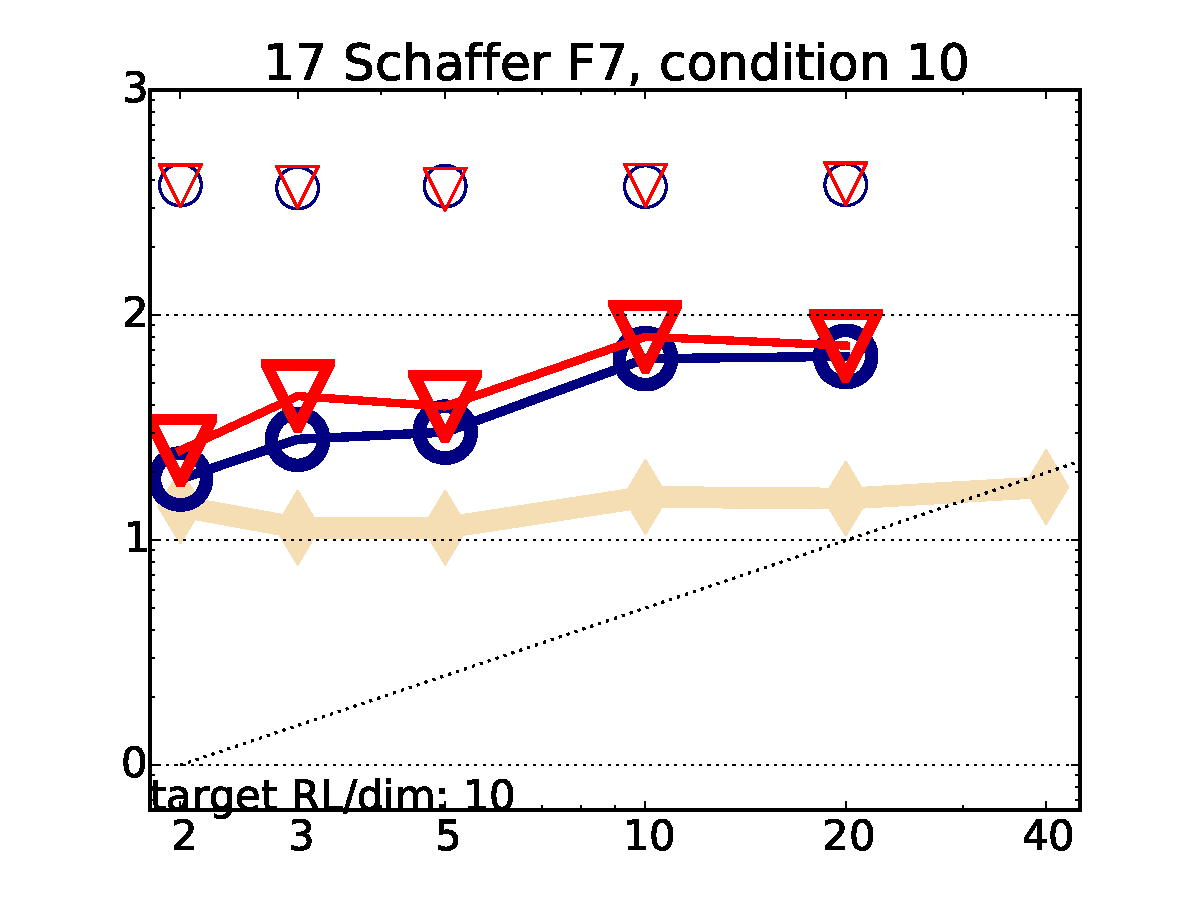
\includegraphics[width=0.253\textwidth, trim= 0.7cm 0.8cm 0.5cm 0.5cm, clip]{ppfigs_f017}&
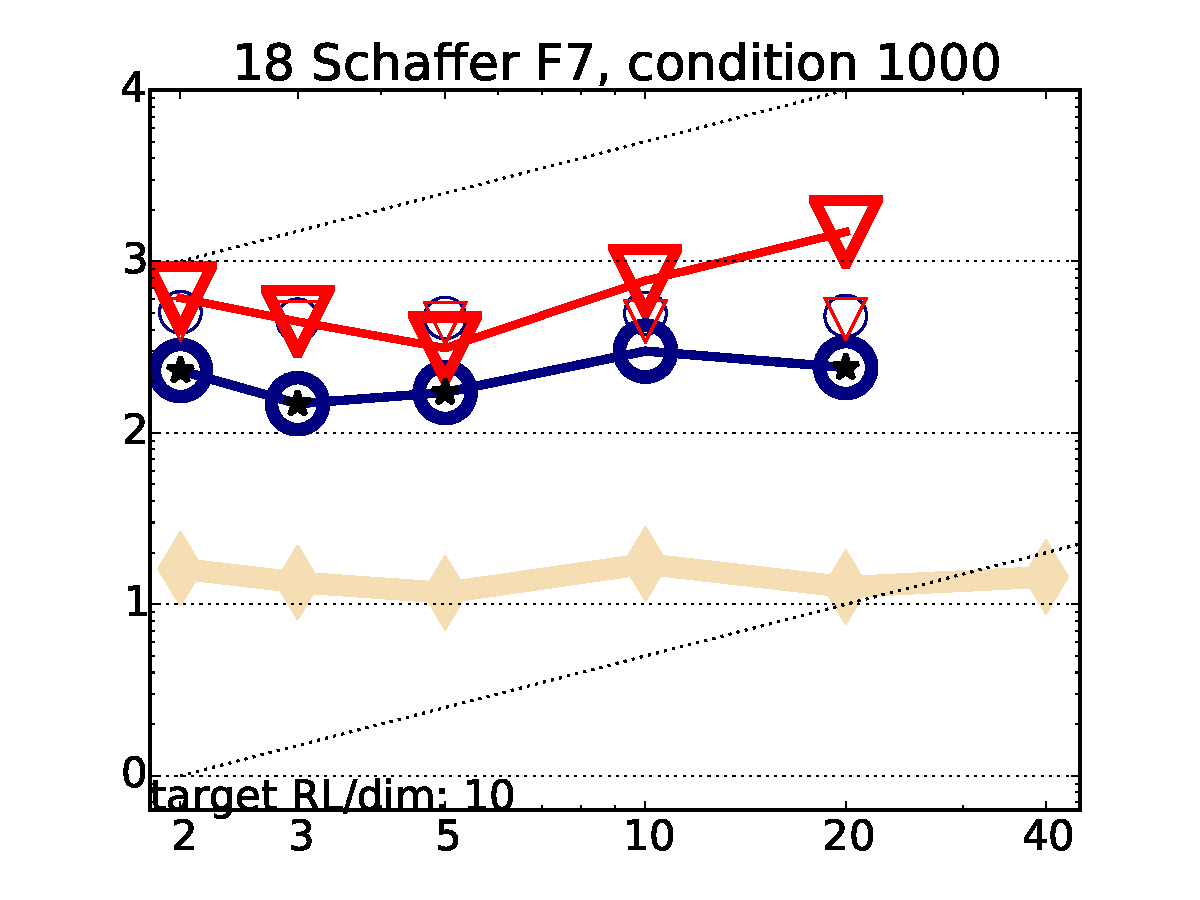
\includegraphics[width=0.238\textwidth, trim= 1.8cm 0.8cm 0.5cm 0.5cm, clip]{ppfigs_f018}&
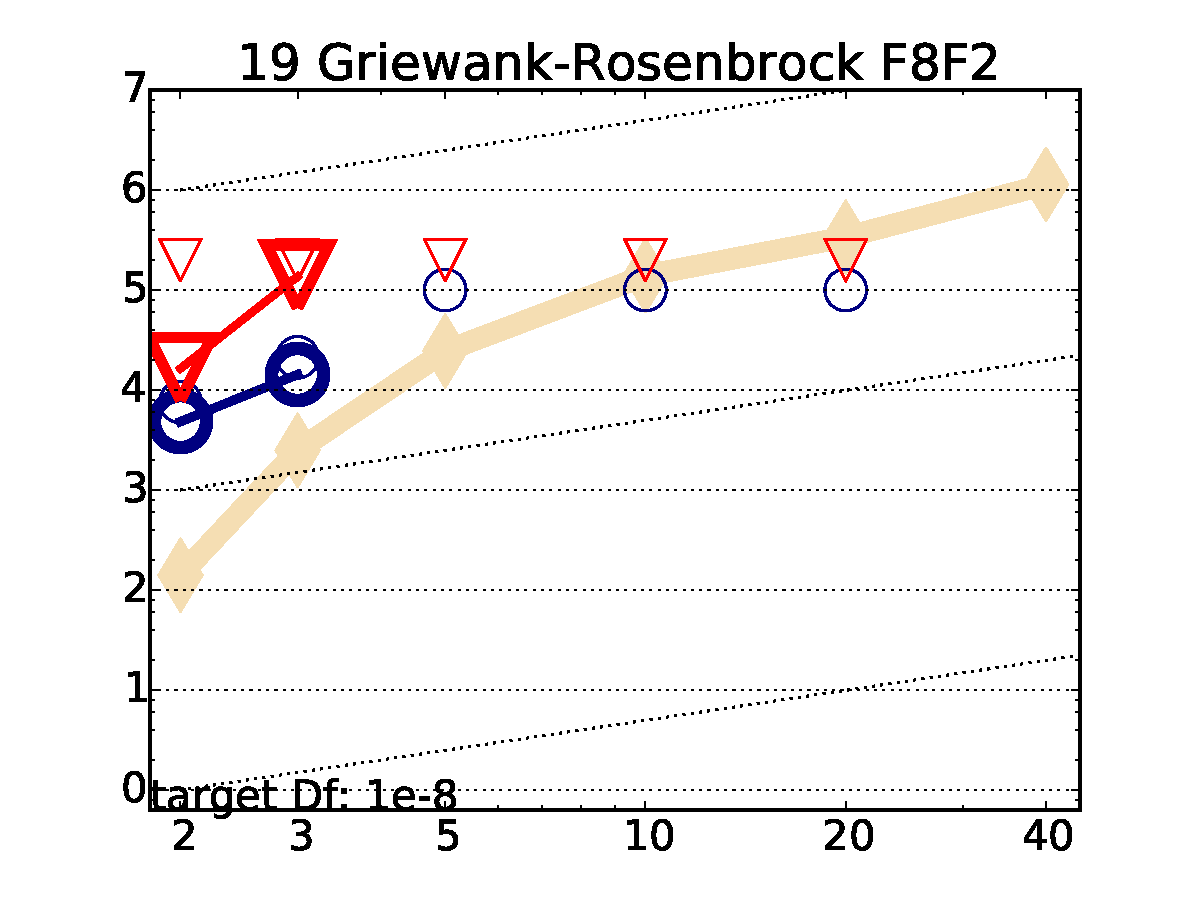
\includegraphics[width=0.238\textwidth, trim= 1.8cm 0.8cm 0.5cm 0.5cm, clip]{ppfigs_f019}&
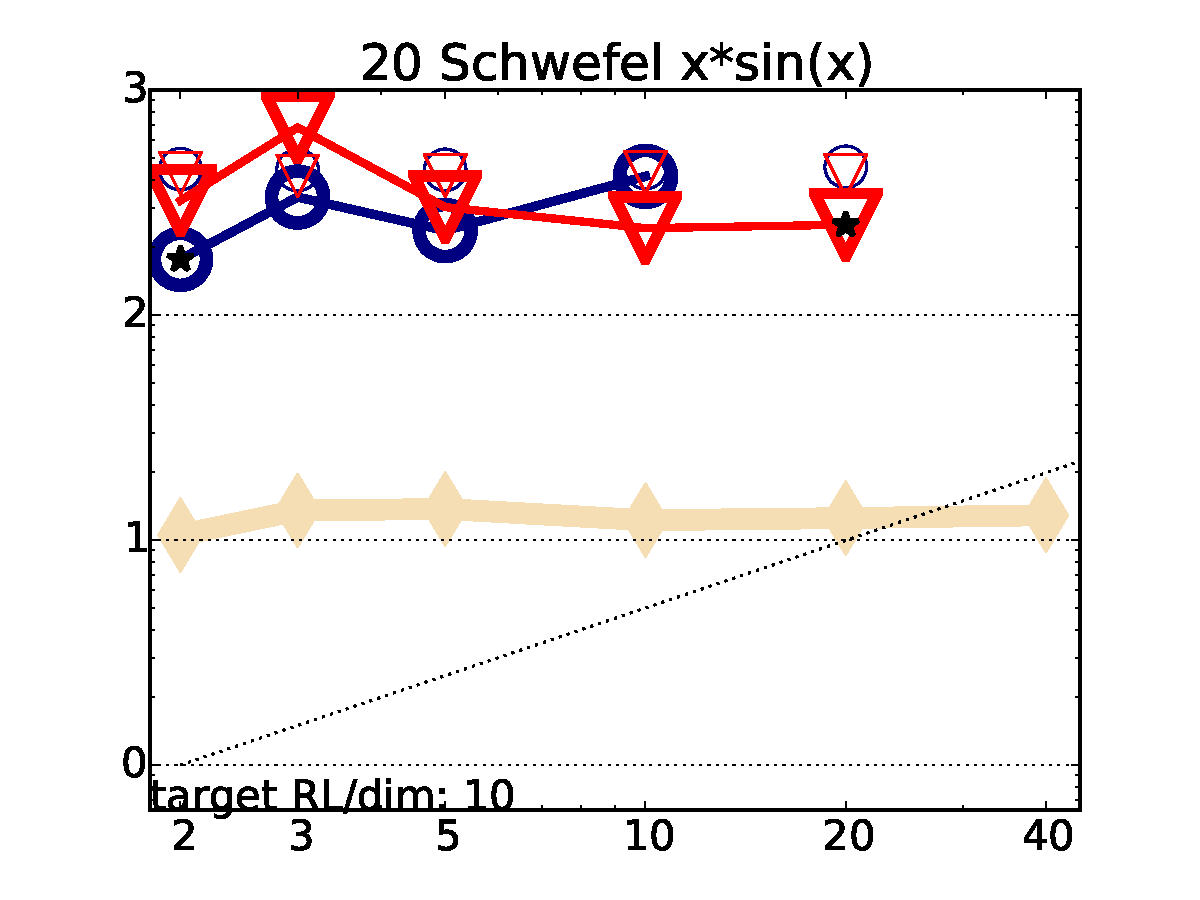
\includegraphics[width=0.238\textwidth, trim= 1.8cm 0.8cm 0.5cm 0.5cm, clip]{ppfigs_f020}\\
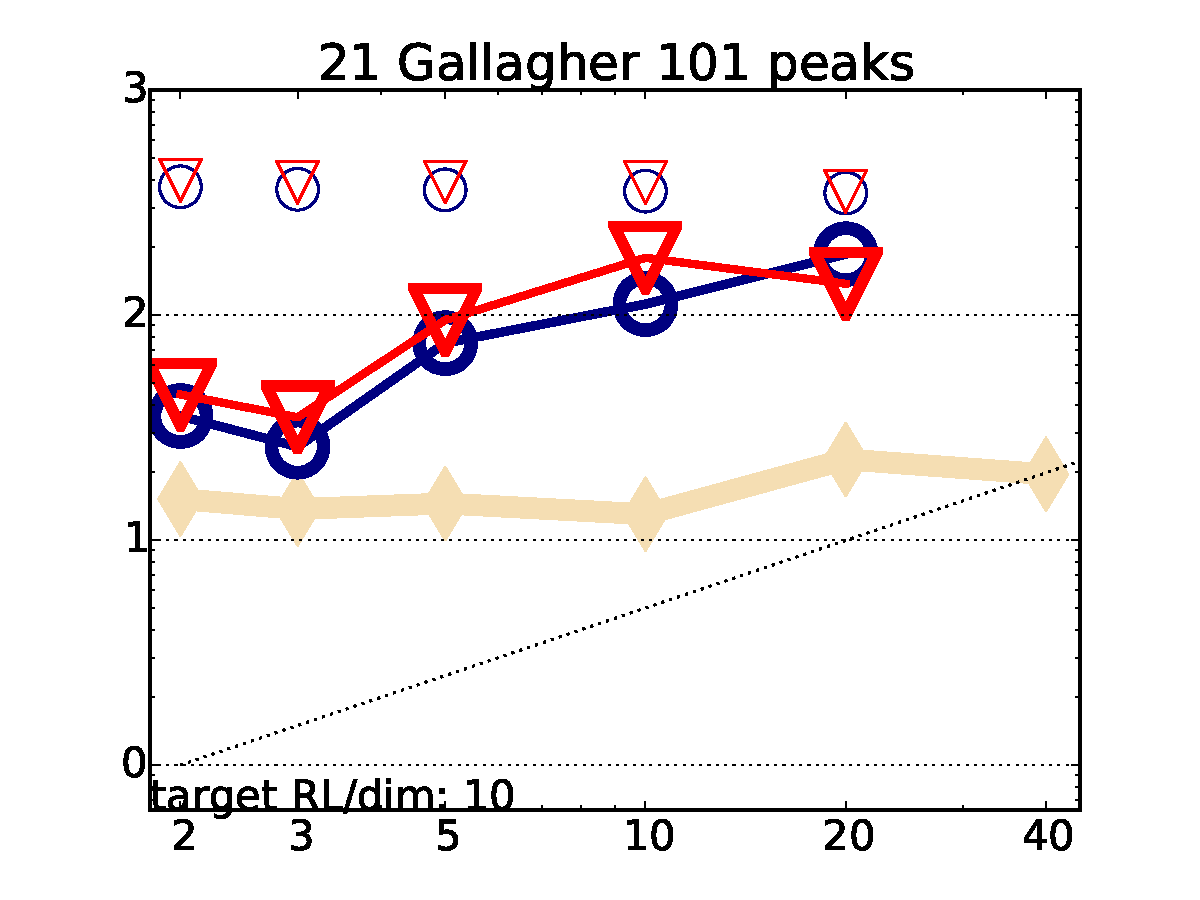
\includegraphics[width=0.253\textwidth, trim= 0.7cm 0.0cm 0.5cm 0.5cm, clip]{ppfigs_f021}&
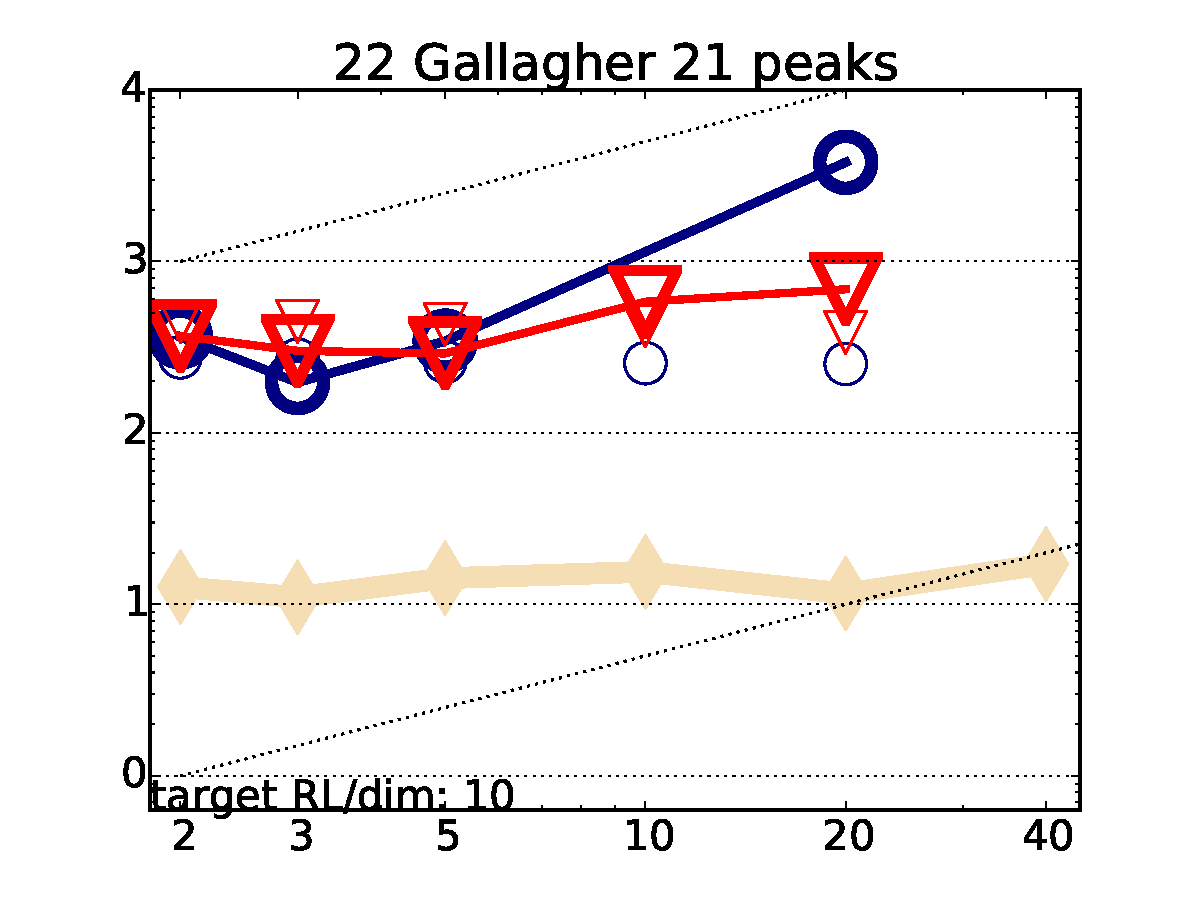
\includegraphics[width=0.238\textwidth, trim= 1.8cm 0.0cm 0.5cm 0.5cm, clip]{ppfigs_f022}&
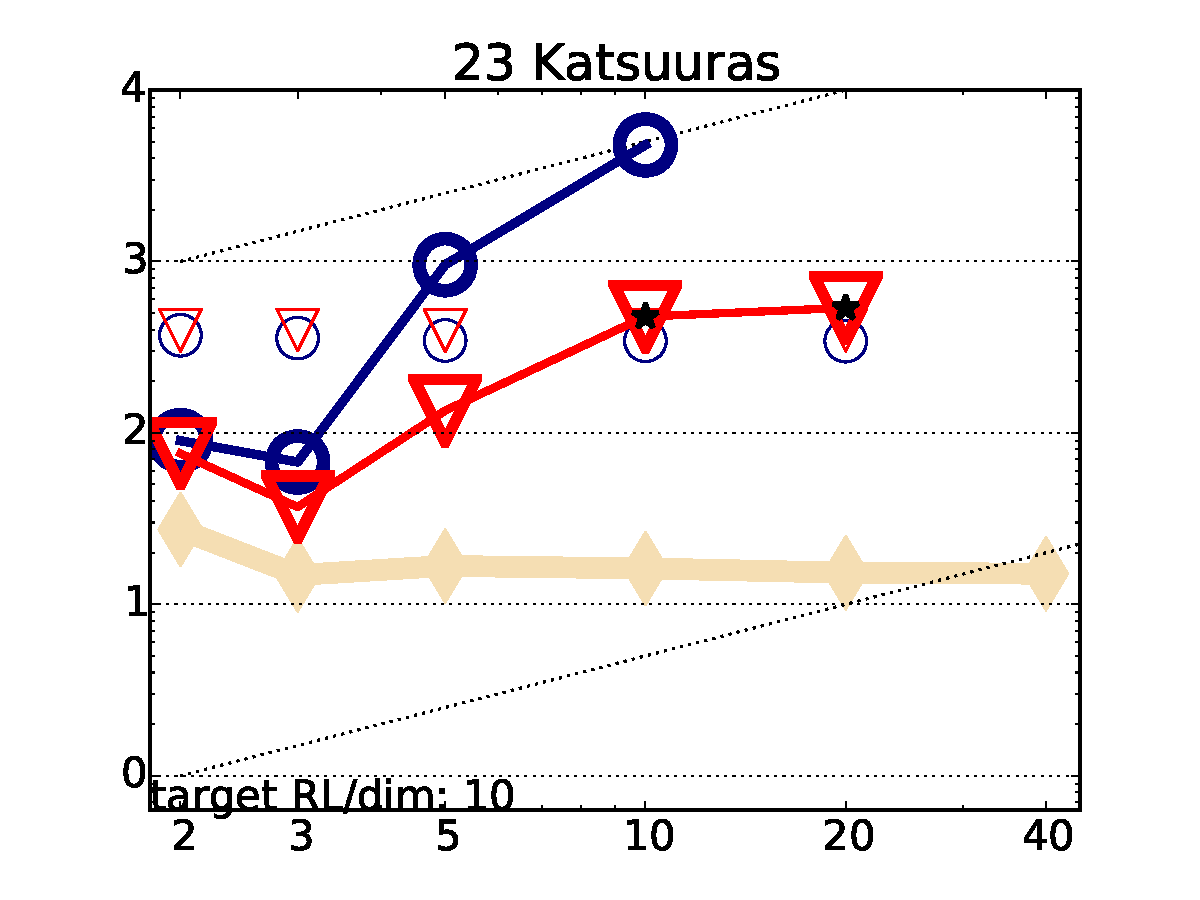
\includegraphics[width=0.238\textwidth, trim= 1.8cm 0.0cm 0.5cm 0.5cm, clip]{ppfigs_f023}&
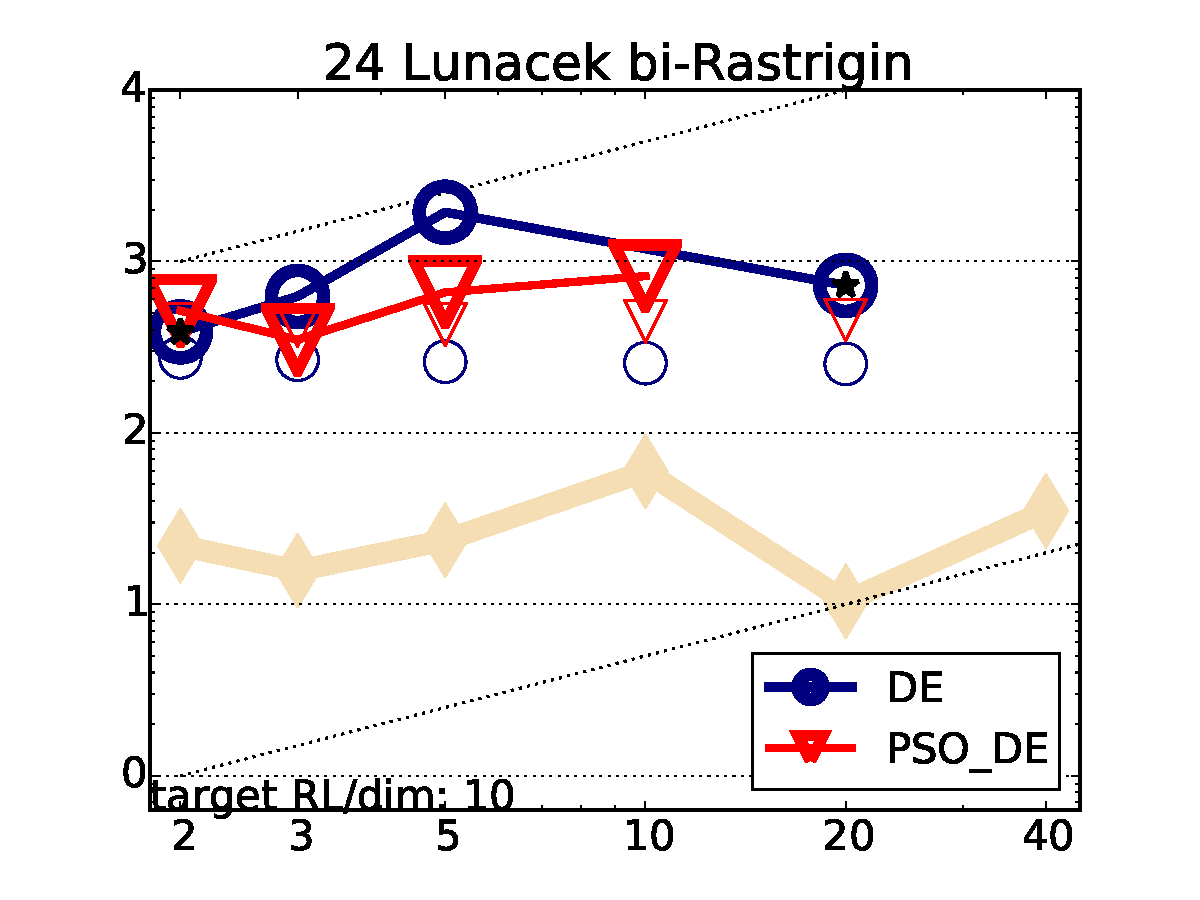
\includegraphics[width=0.238\textwidth, trim= 1.8cm 0.0cm 0.5cm 0.5cm, clip]{ppfigs_f024}
\end{tabular}
\vspace*{-0.2cm}
\caption[Expected running time divided by dimension
versus dimension]{
\label{fig:scaling}
% command defined in bbob_pproc_commands.tex:
\bbobppfigslegend{$f_1$ and $f_{24}$}  % \algorithmA can be defined above, see above
}
% 
\end{figure*}


%%%%%%%%%%%%%%%%%%%%%%%%%%%%%%%%%%%%%%%%%%%%%%%%%%%%%%%%%%%%%%%%%%%%%%%%%%%%%%%
%%%%%%%%%%%%%%%%%%%%%%%%%%%%%%%%%%%%%%%%%%%%%%%%%%%%%%%%%%%%%%%%%%%%%%%%%%%%%%%

% Empirical Cumulative Distribution Functions (ECDFs) per function group
% for dimension 5.

%%%%%%%%%%%%%%%%%%%%%%%%%%%%%%%%%%%%%%%%%%%%%%%%%%%%%%%%%%%%%%%%%%%%%%%%%%%%%%%
\newcommand{\rot}[2][2.5]{
  \hspace*{-3.5\baselineskip}%
  \begin{rotate}{90}\hspace{#1em}#2
  \end{rotate}}
\newcommand{\includeperfprof}[1]{% include and annotate at the side
  \input{\bbobdatapath #1}%
  \includegraphics[width=0.4135\textwidth,trim=0mm 0mm 34mm 10mm, clip]{#1}%
  \raisebox{.037\textwidth}{\parbox[b][.3\textwidth]{.0868\textwidth}{\begin{scriptsize}
    \perfprofsidepanel % this is "\algaperfprof \vfill \algbperfprof \vfill" etc
  \end{scriptsize}}}
}
%%%%%%%%%%%%%%%%%%%%%%%%%%%%%%%%%%%%%%%%%%%%%%%%%%%%%%%%%%%%%%%%%%%%%%%%%%%%%%%
\begin{figure*}
\begin{tabular}{@{}c@{}c@{}}
 separable fcts & moderate fcts \\
 \includeperfprof{pprldmany_05D_separ} &
 \includeperfprof{pprldmany_05D_lcond} \\ 
ill-conditioned fcts & multi-modal fcts \\
 \includeperfprof{pprldmany_05D_hcond} &
 \includeperfprof{pprldmany_05D_multi} \\ 
 weakly structured multi-modal fcts & all functions\\
 \includeperfprof{pprldmany_05D_mult2} & 
 \includeperfprof{pprldmany_05D_noiselessall} 
 \end{tabular}
\caption{
\label{fig:ECDFs05D}
\bbobECDFslegend{5}
}
\end{figure*}


%%%%%%%%%%%%%%%%%%%%%%%%%%%%%%%%%%%%%%%%%%%%%%%%%%%%%%%%%%%%%%%%%%%%%%%%%%%%%%%
%%%%%%%%%%%%%%%%%%%%%%%%%%%%%%%%%%%%%%%%%%%%%%%%%%%%%%%%%%%%%%%%%%%%%%%%%%%%%%%

% Empirical Cumulative Distribution Functions (ECDFs) per function group
% for dimension 20.

%%%%%%%%%%%%%%%%%%%%%%%%%%%%%%%%%%%%%%%%%%%%%%%%%%%%%%%%%%%%%%%%%%%%%%%%%%%%%%%
\begin{figure*}
 \begin{tabular}{@{}c@{}c@{}}
 separable fcts & moderate fcts \\
 \includeperfprof{pprldmany_20D_separ} &
 \includeperfprof{pprldmany_20D_lcond} \\ 
ill-conditioned fcts & multi-modal fcts \\
 \includeperfprof{pprldmany_20D_hcond} &
 \includeperfprof{pprldmany_20D_multi} \\ 
 weakly structured multi-modal fcts & all functions\\
 \includeperfprof{pprldmany_20D_mult2} & 
 \includeperfprof{pprldmany_20D_noiselessall} 
 \end{tabular}
\caption{
\label{fig:ECDFs20D}
\bbobECDFslegend{20}
}
\end{figure*}



%%%%%%%%%%%%%%%%%%%%%%%%%%%%%%%%%%%%%%%%%%%%%%%%%%%%%%%%%%%%%%%%%%%%%%%%%%%%%%%
%%%%%%%%%%%%%%%%%%%%%%%%%%%%%%%%%%%%%%%%%%%%%%%%%%%%%%%%%%%%%%%%%%%%%%%%%%%%%%%

% Expected running time (ERT in number of function evaluations)
% divided by the best ERT measured during BBOB-2009 (given in the respective
% first row) for functions $f_1$--$f_{24}$ for dimension 5.

%%%%%%%%%%%%%%%%%%%%%%%%%%%%%%%%%%%%%%%%%%%%%%%%%%%%%%%%%%%%%%%%%%%%%%%%%%%%%%%
\begin{table*}\tiny
%\hfill5-D\hfill~\\[1ex]
\mbox{\begin{minipage}[t]{0.499\textwidth}\tiny
\centering
\input{\bbobdatapath pptables_f001_05D} 

\input{\bbobdatapath pptables_f002_05D}

\input{\bbobdatapath pptables_f003_05D}

\input{\bbobdatapath pptables_f004_05D}

\input{\bbobdatapath pptables_f005_05D}

\input{\bbobdatapath pptables_f006_05D}

\input{\bbobdatapath pptables_f007_05D}

\input{\bbobdatapath pptables_f008_05D}

\input{\bbobdatapath pptables_f009_05D}

\input{\bbobdatapath pptables_f010_05D}

\input{\bbobdatapath pptables_f011_05D}

\input{\bbobdatapath pptables_f012_05D}

\end{minipage}
\hspace{0.002\textwidth}
\begin{minipage}[t]{0.499\textwidth}\tiny
\centering
\input{\bbobdatapath pptables_f013_05D}

\input{\bbobdatapath pptables_f014_05D}

\input{\bbobdatapath pptables_f015_05D}

\input{\bbobdatapath pptables_f016_05D}

\input{\bbobdatapath pptables_f017_05D}

\input{\bbobdatapath pptables_f018_05D}

\input{\bbobdatapath pptables_f019_05D}

\input{\bbobdatapath pptables_f020_05D}

\input{\bbobdatapath pptables_f021_05D}

\input{\bbobdatapath pptables_f022_05D}

\input{\bbobdatapath pptables_f023_05D}

\input{\bbobdatapath pptables_f024_05D}
\end{minipage}}

 \caption{\label{tab:ERTs5}
 \bbobpptablesmanylegend{dimension $5$}
 }
\end{table*}


%%%%%%%%%%%%%%%%%%%%%%%%%%%%%%%%%%%%%%%%%%%%%%%%%%%%%%%%%%%%%%%%%%%%%%%%%%%%%%%
%%%%%%%%%%%%%%%%%%%%%%%%%%%%%%%%%%%%%%%%%%%%%%%%%%%%%%%%%%%%%%%%%%%%%%%%%%%%%%%

% Expected running time (ERT in number of function evaluations)
% divided by the best ERT measured during BBOB-2009 (given in the respective
% first row) for functions $f_1$--$f_{24}$ for dimension 20.

%%%%%%%%%%%%%%%%%%%%%%%%%%%%%%%%%%%%%%%%%%%%%%%%%%%%%%%%%%%%%%%%%%%%%%%%%%%%%%%
\begin{table*}\tiny
%\hfill20-D\hfill~\\[1ex]
\mbox{\begin{minipage}[t]{0.499\textwidth}\tiny
\centering
\input{\bbobdatapath pptables_f001_20D} 

\input{\bbobdatapath pptables_f002_20D}

\input{\bbobdatapath pptables_f003_20D}

\input{\bbobdatapath pptables_f004_20D}

\input{\bbobdatapath pptables_f005_20D}

\input{\bbobdatapath pptables_f006_20D}

\input{\bbobdatapath pptables_f007_20D}

\input{\bbobdatapath pptables_f008_20D}

\input{\bbobdatapath pptables_f009_20D}

\input{\bbobdatapath pptables_f010_20D}

\input{\bbobdatapath pptables_f011_20D}

\input{\bbobdatapath pptables_f012_20D}
\end{minipage}
\hspace{0.002\textwidth}
\begin{minipage}[t]{0.499\textwidth}\tiny
\centering
\input{\bbobdatapath pptables_f013_20D}

\input{\bbobdatapath pptables_f014_20D}

\input{\bbobdatapath pptables_f015_20D}

\input{\bbobdatapath pptables_f016_20D}

\input{\bbobdatapath pptables_f017_20D}

\input{\bbobdatapath pptables_f018_20D}

\input{\bbobdatapath pptables_f019_20D}

\input{\bbobdatapath pptables_f020_20D}

\input{\bbobdatapath pptables_f021_20D}

\input{\bbobdatapath pptables_f022_20D}

\input{\bbobdatapath pptables_f023_20D}

\input{\bbobdatapath pptables_f024_20D}
\end{minipage}}
 \caption{\label{tab:ERTs20}
  \bbobpptablesmanylegend{dimension $20$}
}
\end{table*}

%%%%%%%%%%%%%%%%%%%%%%%%%%%%%%%%%%%%%%%%%%%%%%%%%%%%%%%%%%%%%%%%%%%%%%%%%%%%%%%
%%%%%%%%%%%%%%%%%%%%%%%%%%%%%%%%%%%%%%%%%%%%%%%%%%%%%%%%%%%%%%%%%%%%%%%%%%%%%%%
%
% The following two commands are all you need in the
% initial runs of your .tex file to
% produce the bibliography for the citations in your paper.
\bibliographystyle{abbrv}
\bibliography{bbob}  % bbob.bib is the name of the Bibliography in this case
% You must have a proper ".bib" file
%  and remember to run:
% latex bibtex latex latex
% to resolve all references
% to create the ~.bbl file.  Insert that ~.bbl file into
% the .tex source file and comment out
% the command \texttt{{\char'134}thebibliography}.
%
% ACM needs 'a single self-contained file'!
%

% \clearpage % otherwise the last figure might be missing
\end{document}
